%!TEX root=../mythesis.tex
% Chapter 1

\chapter{Introduction} % Main chapter title
\chaptermark{Introduction}
\label{ch:introduction} % For referencing the chapter elsewhere, use \ref{Chapter1} 

%----------------------------------------------------------------------------------------
%	SECTION 1
%----------------------------------------------------------------------------------------

\section{Some useful hints}

My figure citation: \fref{fig:demo1}. (command: fref)

My section citation: \sref{sec:contribution}. (command: sref)

My Chaptere citation: \cref{ch:introduction}. (command: cref)

My Paper citation: \cite{bauschke2011convex}. (notice back reference to page from bibliograph)

My equation citation: \eqref{eq:equ2}. (command: eqref), or cite equation by tag: \eqref{eq:equ1}.

\begin{equation}\label{eq:equ1}
F(\theta)=\sum_{i=1}^mf_i(\theta) \tag{DOP}
\end{equation}

\begin{equation}\label{eq:equ2}
F(\theta)=\sum_{i=1}^mf_i(\theta)
\end{equation}

\begin{figure}[htbp]
  \centering
    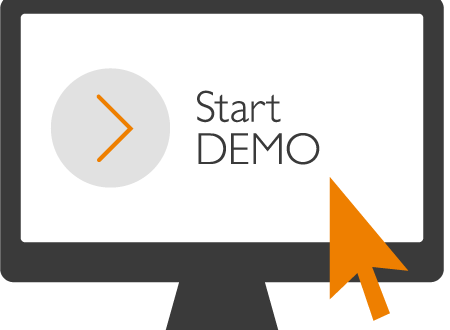
\includegraphics[width=0.85\textwidth]{Chapter1/demo1}
  \caption{An illustration.}
  \label{fig:demo1}
\end{figure}



%----------------------------------------------------------------------------------------
\section{Major Contributions}\label{sec:contribution}
Our main contributions can be stated as follows:
\begin{itemize}
\item \emph{First part}: My first contributions, several lines


\item \emph{Second}: Second contributions, several lines


\item \emph{Third name}: 
Third contributions, several lines

\end{itemize}

%----------------------------------------------------------------------------------------
% SECTION 2
%----------------------------------------------------------------------------------------
\section{Outline of the Thesis}

\cref{ch:introduction} introduces ...

\cref{ch:literature_review} reviews ...



More chapters ....


....

